\documentclass[11pt]{article}
\usepackage{graphicx, color}
\usepackage[margin=1in]{geometry}

%Double-spacing
\renewcommand{\baselinestretch}{2.0}


%\textwidth 16.0cm \textheight 9in %23.5cm
%\oddsidemargin 0.1in
%\evensidemargin 0.1in

\newlength{\figratio}
\setlength{\figratio}{1.0in}1

\newcommand{\centerfig}[2]{
   \centerline{\resizebox{#2in}{!}{\psfig{file=#1.eps}}}}

\title{Artificial Intelligence for Imperfect Information Games  \\
15-300, Fall 2018
}

\author{Author Name Goes Here}
% To remove the date, uncomment the \date{} command below.
%\date{}


\begin{document}
\maket

\section{Introduction}

          	The question of whether machines could develop human-like skills and capabilities has fascinated many great thinkers. One of the founders of computer science, Alan Turing, explored this question in great detail.  Many are aware of the famous Turing Test, a thought-provoking hypothetical game in which a machine attempts to exhibit behavior indistinguishable from a human. While the development of such an Artificial Intelligence is still elusive, many great advancements have been made in matching or surpassing human abilities in more simplified domains.
In particular, games provide a simplified domain that can serve as a benchmark for advancements in Artificial Intelligence. One of Alan Turing’s lesser-known but fascinating contributions to the field was a simple chess-playing program. Computers in Turing’s time lacked the computational power to play chess, so Turing demonstrated this achievement by calculating each move using his program on paper, which took half an hour per move. Less than fifty years later, the famous victory of IBM’s Deep Blue chess computer against Kasparov captured the world’s imagination. In recent years, new advancements in Machine Learning have enabled computers to excel at games with even higher complexity, notably, the success of Google Deepmind’s AlphaGo at the game of Go. Nevertheless, both Go, Chess, and many of the other games which computers have traditionally excelled are all perfect information games, which means that the full state of the game is visible to the players at all times.
This success of artificial intelligence in perfect-information games stands in stark contrast to the real-world environments where humans have to make decisions, where managing and adapting to uncertainty is a defining characteristic. As a result, the development of artificial intelligence for imperfect information games is a critical step towards creating human-like machines. Furthermore, several key advancements in recent years have led to breakthroughs in this field.
          	Perhaps the most famous of all imperfect-information games is Poker and its many variants. The game of Poker has been of significant interest to AI researchers because of its ubiquity, and also the availability of professional human poker players to test their algorithms against. Two of the leading research groups interested in the domain of computer poker are at Carnegie Mellon, led by Tuomas Sandholm and the University of Alberta, led by Michael Bowling. These research groups have been researching computer poker for over a decade. They have developed a wide range of new algorithms and techniques to tackle computer poker. Many of these techniques are highly general, and could be applied to a wide range of sequential imperfect information games.  In addition, these researchers have also benefited from advancements in other areas of computer science. In particular, advances in fast parallel computation using graphical processing units, and also the advent of deep neural networks have aided in achieving several key results.
 

\section{Summary of Paper 1}
\label{ref:paper1-summary}

Here is an example
of how we cite a conference paper by Author1~\emph{et
  al.}~\cite{ConferencePaperExampleTag}.  


\subsection{Approach to solving the problem}
\label{ref:paper1-approach}

\subsection{Summary of results}
\label{ref:paper1-results}

\section{Summary of Paper 2}
\label{ref:paper2-summary}

Here is an example of how we cite
a journal paper by AuthorA~\emph{et al.}~\cite{JournalPaperExampleTag}.

\subsection{Approach to solving the problem}
\label{ref:paper2-approach}

You may want to include illustrations from the papers, if they are helpful,
such as the example shown in Figure~\ref{fig:results-example}.

\begin{figure}[t]
\hrule
\vspace{0.1in}
\centering
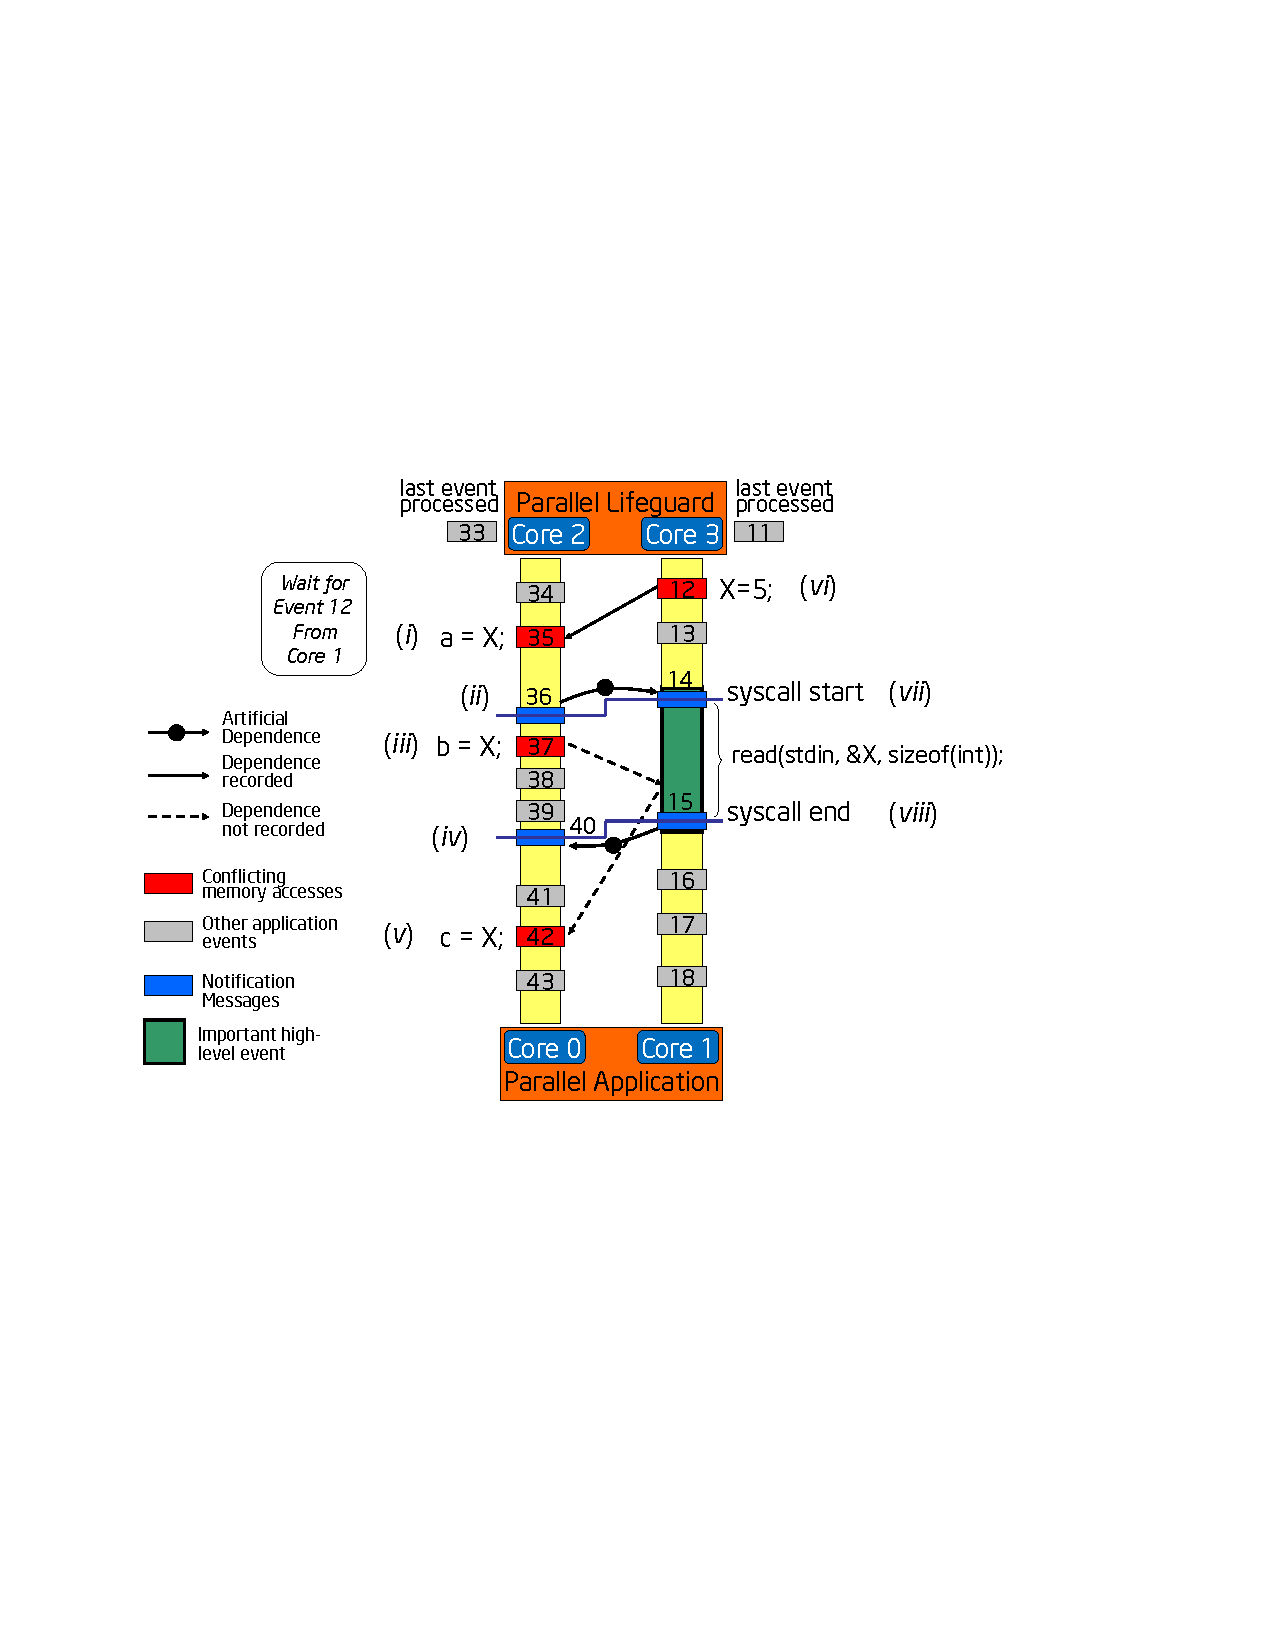
\includegraphics[width=4.0in]{figures/illustration1.pdf}\\
\vspace{0.1in}
\hrule
\caption{Illustration, reproduced from AuthorA~\emph{et al.}~\cite{JournalPaperExampleTag}.}
\label{fig:results-example}
\end{figure}

\subsection{Summary of results}
\label{ref:paper2-results}



\section{Summary of Paper 3}
\label{ref:paper3-summary}

\subsection{Approach to solving the problem}
\label{ref:paper3-approach}

\subsection{Summary of results}
\label{ref:paper3-results}

\section{Comparison of the Three Papers}
\label{ref:comparison-section}

Here you should compare the papers that were discussed earlier in
Sections~\ref{ref:paper1-summary}, \ref{ref:paper2-summary}, and
\ref{ref:paper3-summary}.  You may want to refer back to specific details
in the results sections.  For example, how do the results by
Author1~\emph{et al.}~\cite{ConferencePaperExampleTag} (summarized earlier
in Section~\ref{ref:paper2-results}) compare with the results by
AuthorA~\emph{et al.}~\cite{JournalPaperExampleTag} (summarized above in
Section~\ref{ref:paper1-results}), etc.

\section{Conclusions}
\label{ref:conclusions-section}

What can you conclude from your study?  

\bibliographystyle{plain}
\bibliography{references}

\end{document}

